\documentclass[9pt,conference,compsocconf]{IEEEtran}

\usepackage{hyperref}
\usepackage{amsmath}
\usepackage{graphicx}	% For figure environment
\usepackage{caption}
\usepackage{subcaption}
\usepackage{adjustbox}
\newcommand{\comment}[1]{}

\renewcommand{\thesubfigure}{(\alph{subfigure})}
\captionsetup[sub]{labelformat=simple}

\begin{document}
\pagestyle{plain}
\title{\LARGE{Detecting rooftop available surface for installing PV modules \\ in aerial images using Deep Learning}}

\author{
  Riccardo Cadei, Raphaël Attias, Shasha Jiang \\
  \textit{Department of Computer Science, EPFL, Switzerland} \\
  
  %\small{riccardo.cadei@epfl.ch, raphael.attias@epfl.ch, shsha.jiang@epfl.ch }
}

\twocolumn[
\begin{@twocolumnfalse}
\maketitle

\begin{abstract} 

Mapping the location and size of potential surface on rooftops to install photovoltaics (PV) panels can be a valuable input for policymakers and for investing in distributed energy infrastructures. Machine Learning techniques, combined with satellite and aerial imagery, allow to overcome the limitations of
surveys and sparse databases in providing this mapping at large scale. In this project we apply a supervised method based on convolutional neural networks to delineate available rooftop area for the installation of PV panels by means of pixel-wise image segmentation. We created the dataset from scratch, using satellite images of Genève and labelling them manually. We explored different data augmentation and we varied network parameters in order to maximize model performance. First we trained our model on the whole dataset, then we focused on only on a specific class of images, residential area: our hypothesis is that in order to generalize our solution on new different geographical areas, it is better, in a first step, splitting the dataset in classes (i.e. residential area and industrial area) in a supervised or unsupervised way and then train a different model for each one. Preliminary results show that, training a different model for each area, at the cost of having less data, increases anyway the performance of our detection. In particular we are able to automatically detect, on the residential areas, the available rooftop area at pixel level with an accuracy on the test set of about 0.97 and an Intersection over Union index of 0.77 using only 244 images in the training. The scalability of the trained model should allow to predict the available rooftop area at the Swiss national scale, while new classes (in add to residential and industrial area) could be found to improve and adapt our solution to other country with different  geographic settlement,

\bigskip

\end{abstract}
\end{@twocolumnfalse}
]


\section{Introduction}
Nowadays, people pay more attention to low-carbon development and the use of renewable energy. Installing photovoltaic (PV) panels can effectively lower greenhouse gas emissions and reduce our collective dependence on fossil fuels. Thus, it is extremely useful to detect the available area on a rooftop (ARA) for PV panel installation. In order to automate it, we can use Machine Learning approaches to segment potential PV panel areas on the satellite images. Currently, potential estimation is for the entire rooftop, but our goal here is to obtain an even more precise evaluation of potential areas, where chimneys, windows, existing PV panels and other superstructures are also considered.

As inspired by the automatic detection of rooftop solar panels \cite{castello2019deep} and images segmentation of rooftops \cite{chhor2017satellite}, we developed a Conventional Neural Network model based on U-net \cite{ronneberger2015u}. The model was trained to do binary pixel-wise segmentation on satellite images from Geneva, Switzerland and we aim to generalize our solution on national scale. The labels to predict are binary masks, where the pixels representing ARA are ones, and zero otherwise. By giving a satellite image as input, the output of our model is again a binary image, where the pixels are ones if the probability of representing ARA is bigger than a fixed threshold.


\section{Data Analysis}
\label{sec:dataAnalysis}

\subsection{Data Selection \& Labeling }
\label{subsec:dataSelectionLabeling }
Prefessor Castello Roberto provided us with the satellite images. The dataset was in three folders from three different urban or rural areas in Geneva. Every folder contains 1000 RGB images in PNG form and each image has size $250\times250\times3$ with pixel size $0.25\times 0.25^2$. We selected 657 images randomly among them for our project.
We manually labelled pixels in ARA and non ARA over selected images by a provided tool base on Python. 3 other people helped us label images so we fixed consistent criteria: we used shadow to identify a building and marked the edge the rooftop of the buildings. Superstructures on the rooftops were marked out from the rooftops, eg. the chimneys, windows in the residential areas; pipes, container boxes in the industrial areas. Any other area that is not available to install PV was also excluded. A double check leaves us to hope that the images have been well classified even if sometime the mapping is not trivial even for a human. We tried to label the available areas as precise as possible but it is clear that further efforts in the production of a greater data set will reinforce our research.

Then, as the images looked quite different among them, we manually split the dataset in classes: 257 images in the residential area class, 193 in industrial area class, and the rest 207 images are from non available rooftop area (noARA), where there are not available rooftop areas at all. Since we are not really interest in this last class of images, and they are too easy to predict (all 0s), we dropped all the noARA images except 50 that we consider to reinforce the rejection of false positives,


\subsection{Data prepossessing \& train/validation/test set splitting }
\label{subsec:dataPrepossessing }
Because we have RGB images and colours play an important role in our segmentation task, when loading the dataset, we first saturated them in order to emphasize the contrast of the rooftops with respect to the environment.  After that, we standardized each image with the mean and the variance of the whole dataset, to make sure all data points have the same scale, thus equally important features.

Besides, we tried to adjust the brightness of images, hopefully to support the shadows detection, but it did not seem to improve our detection. Also, we tried to add uniform and gaussian noise to fight overfitting, as our dataset is small, but the accuracy on the validation set did not increase as well.

Finally, we split the data into three sets: 80\% of images for the training, 10\% for the validation and 10\% testing,

\subsection{Data Augmentation}
\label{subsec:dataPAugmentation}
As we have a rather small dataset, we applied a real-time augmentation method only on the training set. 
In model training processing, each time we get an image from the data loader, we randomly flipped it horizontally or flipped it vertically or rotated it in ninety degrees: this increased the dimension of the dataset of a factor 8. After each epoch, all images are used to train, but in every epoch, the images are presented differently. This allowed us to enlarge the dataset without engaging additional memory.
Other techniques of data augmentation were tested, i.e. increasing randomly saturation or brightness, but without evident improvements.

\section{Model}
\label{sec:models}

Starting from an existing model of Convolutional Neural Network developed for biomedical image segmentation, called U-net \cite{ronneberger2015u}, we adapted its architecture for our task, proposing a different training algorithm and loss function and tuning different hyper-parameters. The U-net was shown in \cite{ronneberger2015u} to work well with only a limited number of training examples, provided one made use of data augmentation, and this is exactly our framework.

\subsection{Architecture}
\label{subsec:architecture}
U-net is a Fully Convolutional Network (FCN) divided in two phases: a contracting path which extracts features of different levels through a sequence of convolutions, ReLU activations and max poolings, allowing to capture the context of each pixel ($\italic{encoder}$), and a symmetric expanding path which upsamples the result to increase the resolution of the detected features ($\italic{decoder}$). In the U-net architecture, skip-connections (concatenations) are added between the contracting path and the expanding path, allowing precise localization as well as context. The expanding path therefore consists of a sequence of up-convolutions and concatenations with the corresponding feature map from the contracting path, followed by ReLU activations. To obtain the prediction on an input image, we pass the output of the model in a sigmoid activation function, which gives us for each pixel a probability that it is available for PV installation. Then we take a threshold at 0.5 to label either 0 or 1. 
%(there is not a real need to tune this threshold since the final sigmoid activation function already well separates the 2 classes). 
In Figure \ref{fig:u_net} the original architecture of U-net is presented.

\begin{figure}[h]
    \centering
    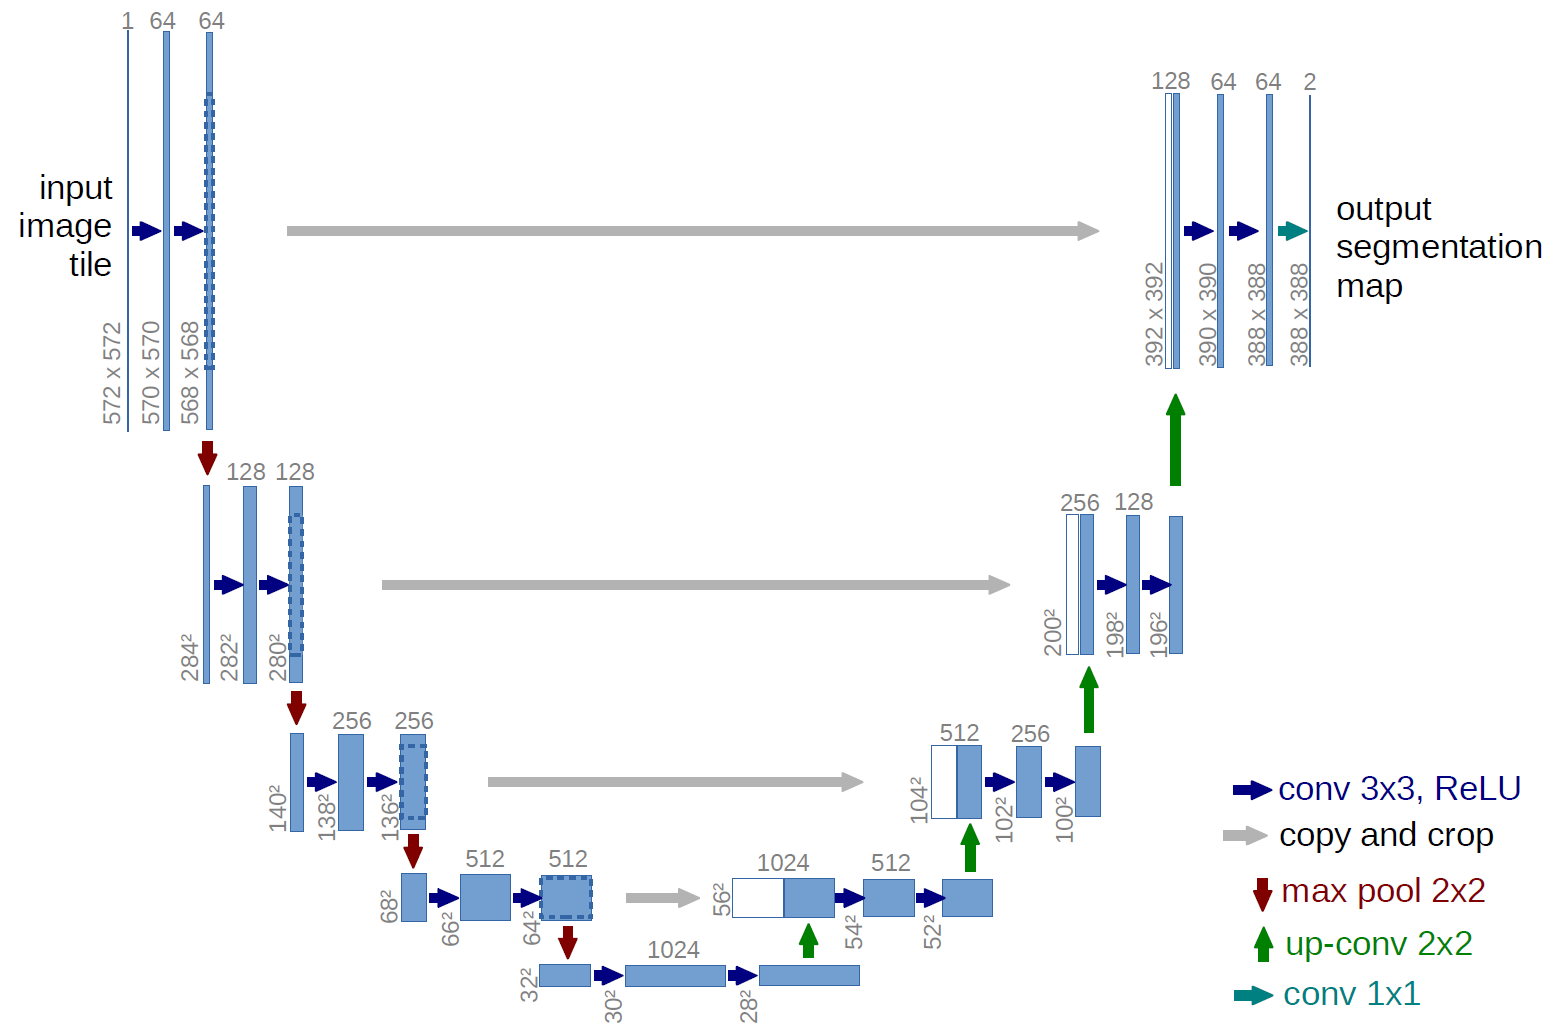
\includegraphics[width=0.4\textwidth]{figures/u_net.png}
    \caption{\footnotesize{U-Net architecture. Each blue box corresponds to a multi-channel feature map. The number of channels is denoted on top of each box. The image pixel size is provided at the lower left edge of the box. White boxes represent copied feature maps. The arrows denote the different operations.}}
    \label{fig:u_net}
\end{figure}

In order to detect rooftop available surface for installing PV modules, we chose to use a slightly modified version of U-Net. First of, we changed the dimensions of the input images to 250 $\cdot$ 250 $\cdot$ 3, as the original U-net was designed for images of size 572 $\cdot$ 572 $\cdot$ 3 and the output to only 1 channel, since we need only the probability of one of the classes (pixel-wise binary classification problem).
Then we modified the padding to ”same” to avoid shrinking when doing convolutions and added batch normalization after each ReLU activation to speed-up training. Inspired by \cite{VariantUNet} we didn't increase the number of channel in the last down-convolution step. We also added dropout in each convolution layer with a rate of 0.1 and 0.2, but since it did not seem to improve the performances we soon took it off: in fact we did not see an evident overfitting while training the model, partly thanks to the use of data augmentation. In general the benefits of using drop out in FCN are not yet very clear and in doubt and short on time to experiment, in agreement with \cite{garbin2020dropout}, we prefer to use only batch normalization. In Figure \ref{fig:u_netbis} we present an our representation of the architecture of our variant of U-Net. In total there are 14'788'929 trainable parameters. 
\begin{figure}[h]
    \centering
    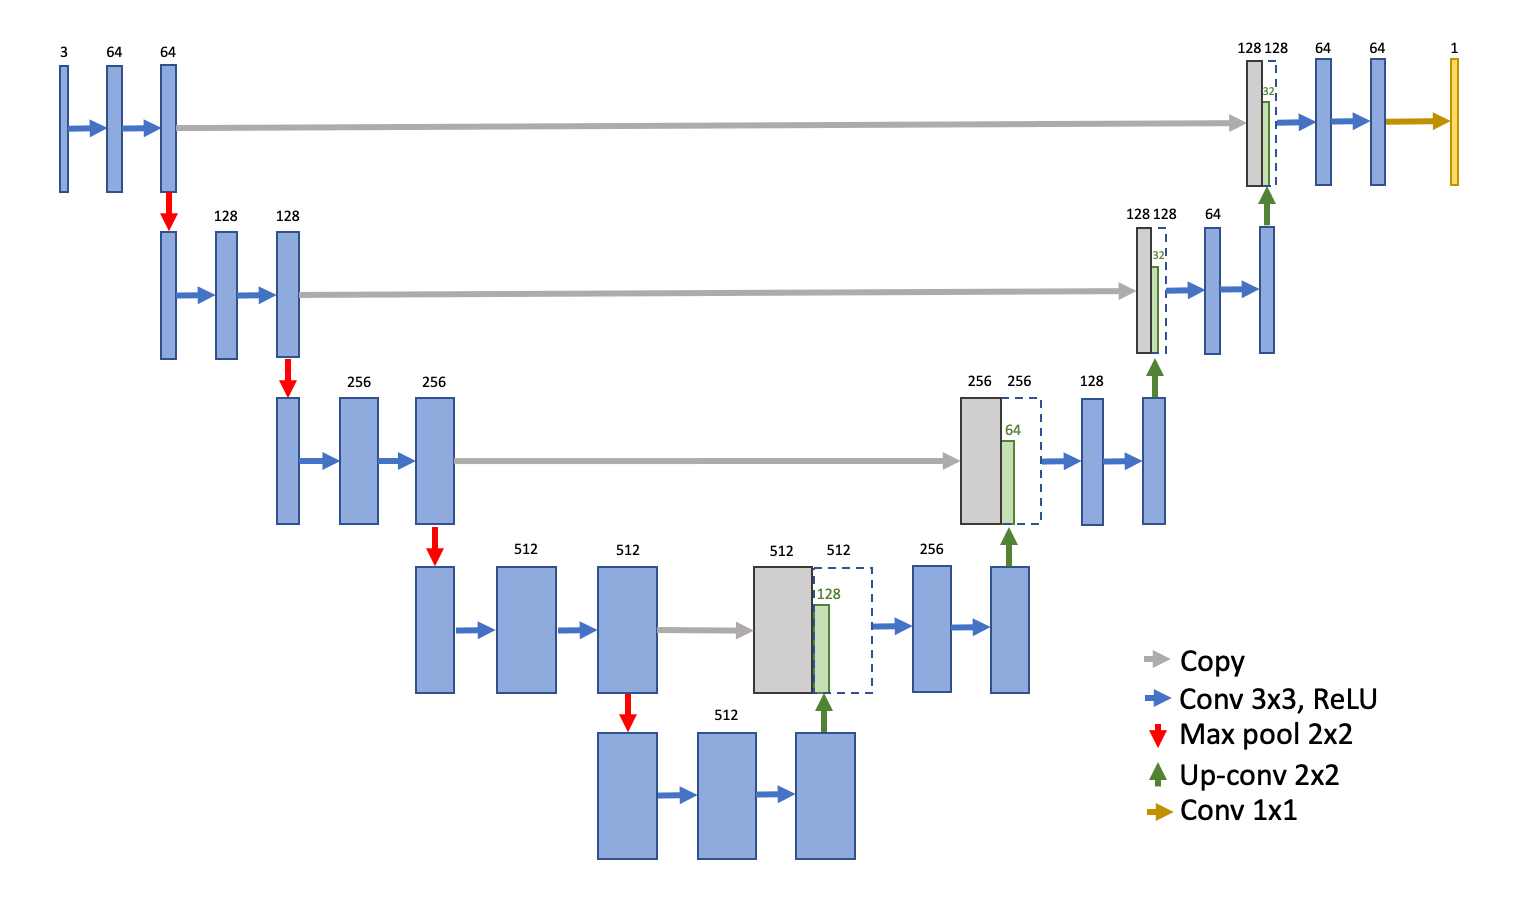
\includegraphics[width=0.4\textwidth]{figures/arch.png}
    \caption{\footnotesize{Variant of U-Net architecture used in this project. We can observe the padding added after each upconv to obtain a final output with the same dimensions as the input. The output is only 1 channel, we need the probability of one of the classes since this is a pixel-wise binary classification problem. Finally we can note that the last downconv block does not increase the number of channels.}}
    \label{fig:u_netbis}
\end{figure}


\subsection{Training}
\label{subsec:training}

We do not start from a pre-trained model; hence we train the algorithm starting from a random set of
weights, using batches of 5 images from the training set (higher batch size is not supported in terms of memory on our machine).

Since our data set is quite unbalanced (more not ARA pixels than ARA), as in  \cite{castello2019deep}, we propose a weighted pixel-wise categorical cross entropy loss function: 

\begin{multline}
    L(\textbf{x,y}) = - \frac{1}{N \cdot |I|} \sum_{n=1}^{N} \sum_{i  \in I} w_n [ p_c y_{n,i} \cdot \log \sigma(x_{n,i}) & + (1 - y_{n,i}) \cdot \log (1 - \sigma(x_{n,i})) ]
\end{multline}

computing the mean of the weighted entropy loss over all the pixels $i \in I (= \{1,..., 250\}^2)$ of all the $N(=5)$ images of a batch. We assign larger weight $p_c$ to the false negative loss (predicting ARA instead of no-ARA) and we combine the final Sigmoid layer and the loss in one single class. This version is more numerically stable \cite{BCEWITHLOGITSLOSS:2019} than using a plain Sigmoid followed by a loss as, by combining the operations into one layer, we take advantage of the log-sum-exp trick.

In order to evaluate the final performances of our model we consider two metrics: the $Accuracy$ and  the $Jaccard$ $index$, as known as intersection over union ($IoU$). Given two set A,B, in our task representing the pixels predicted as ARA in an image and the real ARA pixels, we define:

$$
IoU(A,B)=\frac{|A \cap B|}{|A \cup B|}
$$


Evaluate the $Accuracy$ is a standard in Supervised Learning tasks, however when the data set is unbalanced, and this is the case, it becomes a too optimistic metric to evaluate the performance of a model since classify the elements of the bigger class it is easier. $IoU$ is a standard in Image Segmentation and by definition can manage unbalanced dataset: somehow it expresses how much the object detected is complete or not. For this reason we focus on $IoU$ in order to evaluate the performance of our model. In literature $IoU>0.5$ is considered a good prediction. 

For this reason, we tuned the value of $p_c$ in the loss using Grid Search maximizing the $IoU$ on the validation test.

We replaced the Stochastic Gradient Descent with the Adam Optimizer, known to converge faster during training \cite{kingma2014adam} and we combined it decreasing the learning rate of each parameter group by $\gamma$ every $step\_size$ epochs. Using a decreasing learning rate allowed our loss function to converge during the train, fact that we didn't get it before. To be honest this adding came from an error, but it is known life's greatest lessons are usually learned at the worst times and from the fundamental mistakes.
In particular we were running a Grid Search (using Cross Validation) to evaluate the best constant learning rate for Adam, proposing a list of decreasing values. We forgot to reset the weights of the model after each training, but the surprising result was that the loss function converged, for the first time, and the final model was predicting with the right criteria (even if without excellent performances). As we discovered our error we replicated this involuntary huge adaptive learning  directly decreasing the learning rate of each parameter group by $\gamma$ every $step\_size$ epochs.
We tuned the initial learning rate, $\gamma$ and $step\_size$ through Grid Search (this time correctly resetting the weights of the model at each iteration) maximizing the $IoU$ on the validation test. Training was done on our personal GPU, a Nvidia GTX 1660 with 6 GB of VRAM.




\section{Results}
\label{sec:results}
\subsection{Model on full training set}
\label{subsec:full}
First we trained the model described in section \ref{subsec:architecture} on the entire training set equal to the 80\% of 257 residential, 193 industrial and 50 NoARA images. As the quality of labelling on the industrial areas is worse because of their complex structures, we expected a lower $IoU$ on this full training set. Setting the initial learning rate to $0.1$, the $(\gamma,step)$ parameters of the scheduler to $(0.8,60)$, we trained for $1000$ epochs to decide where should we stop the training for the final model, avoiding to overfit. We observed that after 225 epochs, our model had the best balance of low loss and high $IoU$ on validation set, before to start to get worse. Retraining with the optimal number of epochs (225) we obtained a final loss on the val set of $0.8702$, and an $IoU$ of $0.6121$ again on the val set. On the test set, the $IoU$ obtained is $0.5886$. Figure \ref{fig:full_loss_iou} shows the evolution of the loss and $IoU$ with respect to the number of epoch during the training.

\begin{figure}[h!]
    \centering
     \begin{subfigure}[b]{0.23\textwidth}
         \centering
        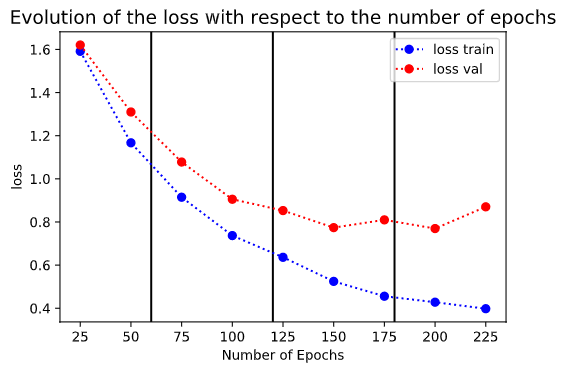
\includegraphics[width=\textwidth]{figures/loss200_batch5loss4.png}
        %\caption{Evolution of the loss with respect to the number of epoch, on the train set or validation set. We can observe that at iteration $x$, we minimized the loss on validation set.}
        \label{fig:full_loss}
     \end{subfigure}
     \hfill
     \begin{subfigure}[b]{0.23\textwidth}
         \centering
        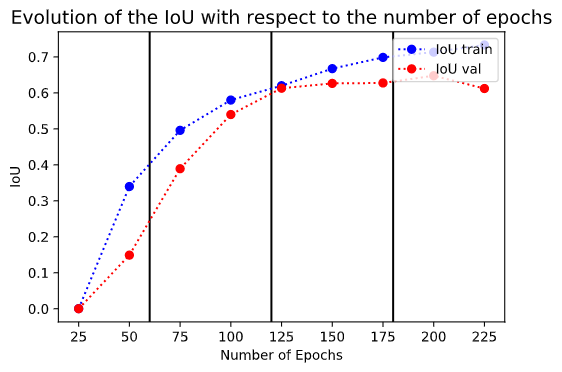
\includegraphics[width=\textwidth]{figures/iou200_batch5loss4.png}
       % \caption{Evolution of the $IoU$ with respect to the number of epoch, on the train set or validation set. Again we observe that at iteration $x$, we maximizes the $IoU$ metric on the validation set.}
        \label{fig:full_loss}
     \end{subfigure}
 \caption{\footnotesize{Evolution of the loss and $IoU$ with respect to the number of epoch, on the train set or validation set. We can observe that at iteration $x$, we minimized the loss and $IoU$ on validation set.}}
 \label{fig:full_loss_iou}
\end{figure}

In Figure \ref{fig:pred_full} we present some predictions outputted by this model on the testing data.

\begin{figure}[h!]
    \centering
    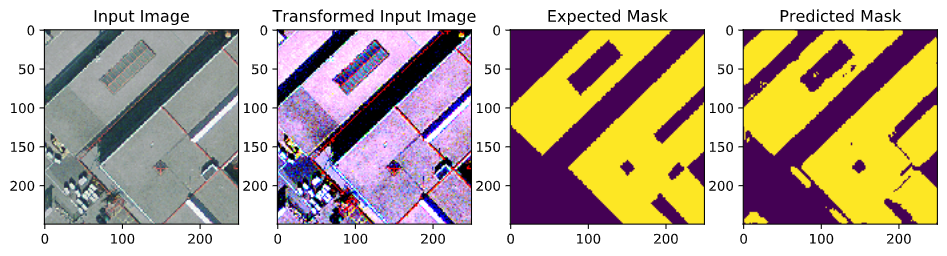
\includegraphics[width=0.45\textwidth]{figures/pred_full_1.png}
    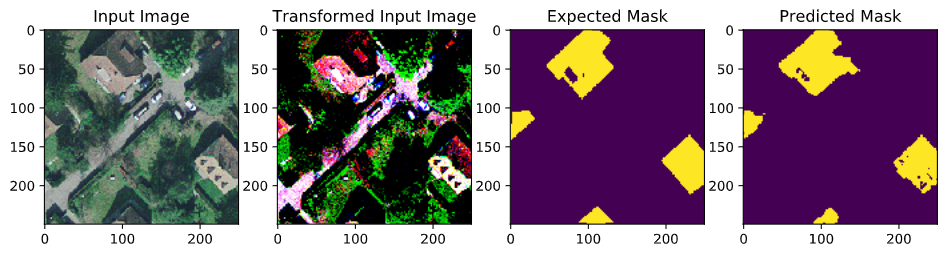
\includegraphics[width=0.45\textwidth]{figures/pred_full_2.png}
    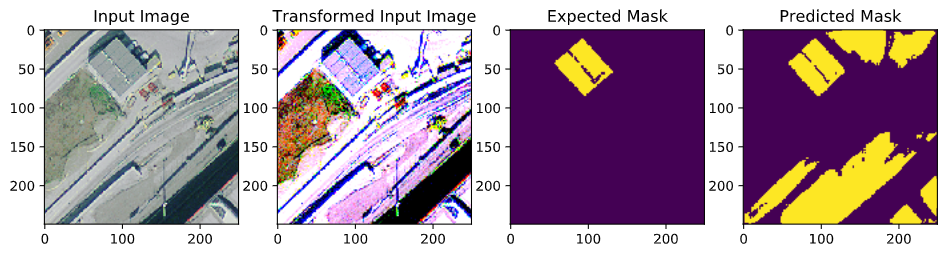
\includegraphics[width=0.45\textwidth]{figures/pred_full_3.png}
    \caption{\footnotesize{3 examples of prediction on images from the test, by the model trained on 225 epochs on the entire training set (industrial \& residential images).}}
    \label{fig:pred_full}
\end{figure}

While the model seems to perform adequately in average on the test set, we observed some predictable behaviors. The model trained on the full training set seems to perform well on residential areas but poorly on industrial areas. This could be explained my multiple factors, first the buildings in residential areas are mostly small rectangular shaped buildings, with easily distinguishable rooftop structures. This is in opposition to industrial buildings, where the buildings can fill the entire image, or the complexity of some additional structures are detrimental to the performance of the algorithm. Secondly the model could be confused from so different structure to detect.
We deduced then that it may be beneficial to train a different model for each specific class at time and we focused only on the segmentation of satellites images from residential areas. Before moving on we summarize in Table \ref{fig:my_label} the performances of our network on this first problem.

\begin{table}[h!]
    \centering
    \begin{tabular}{ |c|c|c|c| } 
\hline
Data Set & IoU & Accuracy \\
\hline
Train Set & 0.7244 & 0.9534 \\ 
Validation Set & 0.6121 & 0.9108 \\ 
Test Set & 0.5886 & 0.9202 \\ 
\hline
\end{tabular}
    \caption{\footnotesize{IoU and Accuracy and our three data sets, for the model trained on 225 epochs on the entire training set.}
    \label{fig:my_label}}
\end{table}

\subsection{Model on residential training set}
We trained a new network in a similar framework than the previous subsection just considering only the 257 residential area images (+ 50 NoARA to reinforce the rejection of false positives). Firstly we trained the model for 1000 epochs with an initial learning rate of $0.2$ for the optimizer, with $(0.8,60)$ parameters for the scheduler of the adaptive learning. We found that 300 epochs of training are enough, as the IoU on the validation set reaches its maximum and the loss on the validation set is around its minimum. So, fixed these hyper-parameters, we performed a grid-search on the best weight for the binary cross entropy loss, ranging from 4 to 7. The right loss weight should allow us to counter the unbalanced nature of our pixel-wise classification problem. Then we retrain the network with all the optimized hyper-parameters and the evolution of the IoU and the loss with respect to the epochs is shown in Figure \ref{fig:residencial_plots}. 

\begin{figure}[h!]
    \centering
     \begin{subfigure}[b]{0.23\textwidth}
         \centering
        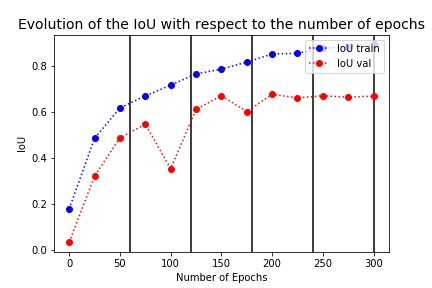
\includegraphics[width=\textwidth]{figures/iou_batch5loss6.png}
        %\caption{Evolution of the loss with respect to the number of epoch, on the train set or validation set. We can observe that at iteration $x$, we minimized the loss on validation set.}
     \end{subfigure}
     \hfill
     \begin{subfigure}[b]{0.23\textwidth}
         \centering
        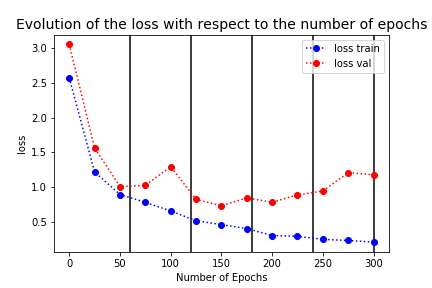
\includegraphics[width=\textwidth]{figures/loss_batch5loss6.png}
       % \caption{Evolution of the $IoU$ with respect to the number of epoch, on the train set or validation set. Again we observe that at iteration $x$, we maximizes the $IoU$ metric on the validation set.}
     \end{subfigure}
\caption{\footnotesize{Evolution of the loss and $IoU$ with respect to the number of epoch, on the train set or validation set in residential areas. We can observe that at iteration $300$, the IoU seems to be stabilized on the validation set and we obtain a satisfactory loss on the train set.}
\label{fig:residencial_plots}}
\end{figure}

In Figure \ref{fig:residencial_pred} we present some predictions on the testing data outputted by this new specific model for residential area.

\begin{figure}[h!]
    \centering
    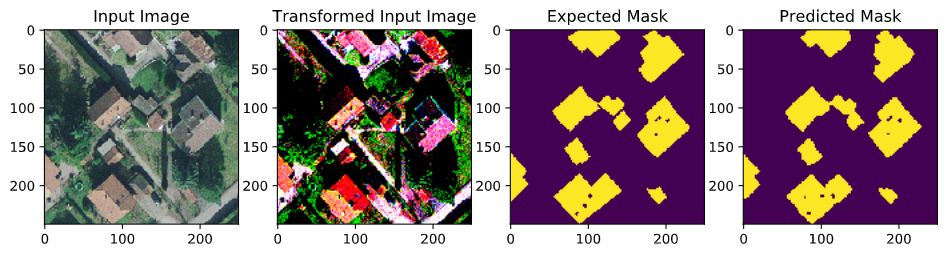
\includegraphics[width=0.45\textwidth]{figures/pred_residencial_1.png}
    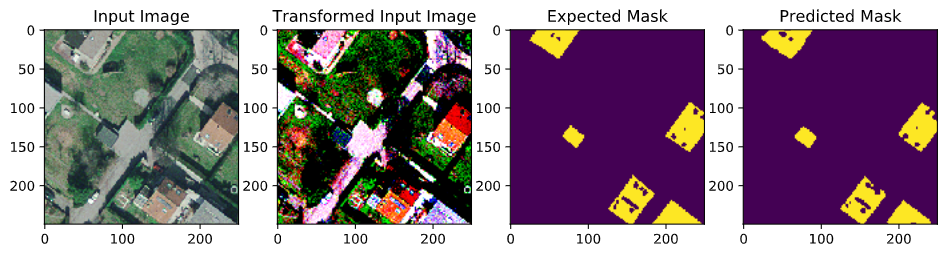
\includegraphics[width=0.45\textwidth]{figures/pred_residencial_2.png}
    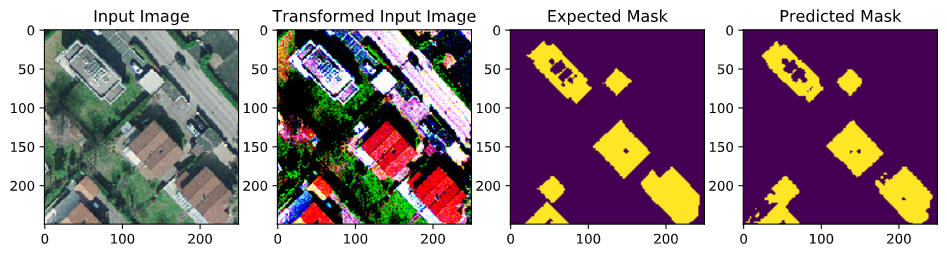
\includegraphics[width=0.45\textwidth]{figures/pred_residencial_3.png}
    \caption{\footnotesize{3 examples of prediction on images from the test, by the model trained on 300 epochs on the residential training set.}}
    \label{fig:residencial_pred}
\end{figure}

We can observe that comparing with the residential area images of the test set of the general model, this new predictions are more precise, even if trained with almost half of the images. The details are sharper and we can see that now we can successfully detect hyper construct on the rooftops, like chimneys or windows, and does not label incorrectly neighboring objects like roads, gardens or cars. 
%From Figure \ref{fig:residencial_plots}, we observe that at 300 epochs the loss on validation is 1.1786, and the IoU is 0.6686. 
On the test set, we obtained a $IoU$ of 0.7756 and an $Accuracy$ of 0.9708. This improvement confirms the hypothesis we have made at the end of subsection \ref{subsec:full}, that the training on industrial areas is detrimental to the prediction of residential areas. In Table \ref{fig:my_labelres} we summarize the results of this specific model for residential area. 

\begin{table}[h!]
    \centering
    \begin{tabular}{ |c|c|c|c| } 
\hline
Data Set & IoU & Accuracy \\
\hline
Train Set & 0.9006 & 0.9863 \\ 
Validation Set & 0.6686 & 0.9536 \\ 
Test Set & 0.7756 & 0.9708 \\ 
\hline
\end{tabular}
    \caption{\footnotesize{IoU and Accuracy and our three data sets, for the model trained on residential areas for 300 epochs.}
    \label{fig:my_labelres}}
\end{table}

The difference of $IoU$ between validation and train is due to the only few images ($\approx$ 30) that we are considering for each set and the difference of difficulty of the detection task among different images. A greater dataset should annul this difference.

\section{Prospects}
From our work on this segmentation problem, we learnt and understood how important the quality of a dataset is. We came up with solutions to counter this problem with our data augmentation techniques, but the poor results on some samples in industrial areas were indicative of this problem. In some further work, one could try to first implement a classifier or an unsupervised learning algorithm to split the dataset in clusters and train a different model for each cluster. Our suspect is that, even if different geographical region can't be split in the same classes, a model for a fixed class (i.e. residential area) should generalize even between different countries.
Another solution suggested for further research is to apply on the output of the model a graph cut algorithm to remarkably improves the edges of the segmented buildings. While this algorithm may make detecting hyper structure more difficult, it has been shown to be an efficient solution to make the final output clearer \cite{rs9070701}.

\section{Conclusion}

In this project, we examined an end-to-end approach for semantic segmentation of satellite images for available rooftop are to install PV panels detection using few data, and with a relatively low resolution.
We proposed a CNN based on the U-net architecture proposing a different training  algorithm  and  loss  function  and  tuning  different  hyper-parameters.
We created the dataset from scratch, labelling 657 satellite images and we compared several techniques of data transformation and data augmentation. We further split the problem for a specific geographical settlement: residential area. Both on the whole dataset and with a specific focus on residential area we achieved IoU and accuracy at state-of-the-art results for comparable task \cite{castello2019deep}, \cite{chhor2017satellite}. In particular for residential area we got an $Accuracy >0.97$  and  an $IoU >0.77$  using  only  244  images  in  the  training. The scalability  of  the  trained  model  should  allow us  to  predict  the  available  rooftop  area  at  the  Swiss  national  scale,  while  new  classes  (in  add  to residential and industrial area) could be found in order to improve and adapt our solution to other countries with different geographic settlements.

\twocolumn[
\begin{@twocolumnfalse}
\nocite{*}
\bibliographystyle{IEEEtran}
\bibliography{literature}
\end{@twocolumnfalse}
]


\end{document}
